\documentclass{article}
\usepackage{graphicx}
\usepackage{listings}
\usepackage{xcolor}
\usepackage{hyperref}
\usepackage{url}
\usepackage{amsmath}
\usepackage{braket}
\usepackage{amsfonts}
\title{Quantum Gates: The Building Blocks of Quantum Computing}
\author{Emir Kaan Özdemir}
\date{September 2024}

\lstset{
  language=[Sharp]C, % I had to use C# because there was no Q# option
  basicstyle=\ttfamily\small,
  keywordstyle=\color{blue},
  stringstyle=\color{orange},
  commentstyle=\color{gray},
  numbers=left,
  numberstyle=\tiny\color{gray},
  stepnumber=1,
  numbersep=10pt,
  backgroundcolor=\color{lightgray!10},
  tabsize=2,
  breaklines=true,
  breakatwhitespace=false,
  showspaces=false,
  showstringspaces=false
}


\begin{document}

\maketitle

\begin{abstract}
    Quantum gates, pivotal to the functioning of quantum computers, represent the quantum counterpart to classical logic gates but operate on entirely different principles. Unlike classical gates that process binary bits, quantum gates manipulate qubits, enabling operations that harness quantum phenomena such as superposition and entanglement. These operations allow quantum computers to perform calculations that would be intractable for classical systems. This paper explores the significance of quantum gates in quantum algorithm development, their unique capabilities compared to classical gates, and their potential impact on various fields, including cryptography, optimization, and artificial intelligence. The content is structured to be accessible, but a solid understanding of advanced mathematical concepts may be necessary. 
\end{abstract}

\vspace{7cm}

\tableofcontents

\vspace{13cm}

\section{Introduction}
Quantum gates are fundamental components in the realm of quantum computing, analogous to classical logic gates in traditional computers. However, their function and impact reach far beyond classical computation, enabling quantum computers to perform complex operations that are impossible for classical systems. This article explores the critical role quantum gates play in the development of quantum algorithms, their differences from classical gates, and their potential to revolutionize fields such as cryptography, optimization, and artificial intelligence. Although it is aimed to explain all of these in a simple and clear manner, more than a high school level of mathematics may be required to understand comfortably. Knowledge of complex numbers is required. Mathematical expressions and code snippets will be explained. The Q\# programming language used for code blocks.

\vspace{3cm}

\section{Necessary Mathematical Expressions}

\subsection{Matrices, Vectors and Scalars}
\subsubsection{Matrices(Matrix)}
A matrix is set of numbers arranged in a rectangular grid. Here is a 2 by 2 matrix:
\begin{equation*}
    A = \begin{bmatrix} 1 & 2 \\ 3 & 4 \end{bmatrix}
\end{equation*}
The notation $A_{i,j}$ refers to the element in row i and column j of matrix A(all indices are 0-based). In the above example, $A_{0,1} = 2$.

An $n \times m$ matrix will have n rows and m columns:
\begin{equation*}
    \begin{bmatrix}
    x_{0,0} & x_{0,1} & \dotsb & x_{0,m-1} \\
    x_{1,0} & x_{1,1} & \dotsb & x_{1,m-1} \\
    \vdots  & \vdots  & \ddots & \vdots  \\
    x_{n-1,0} & x_{n-1,1} & \dotsb & x_{n-1,m-1}
\end{bmatrix}
\end{equation*}
Quantum computing uses complex-valued matrices: the elements of a matrix can be complex numbers. This, for example, is a valid complex-valued matrix:
\begin{equation*}
    \begin{bmatrix}
    1 & i \\
    -2i & 3 + 4i
\end{bmatrix}
\end{equation*}

\subsubsection{Vectors(Vector)}
A vector is an $n \times 1$ matrix. Here, for example, is a $3 \times 1$ vector:
\begin{equation*}
    V = \begin{bmatrix} 1 \\ 2i \\ 3 + 4i \end{bmatrix}
\end{equation*}
Since vectors always have a width of 1, vector elements are sometimes written using only one index. In the above example, $V_0 = 1$ and $V_1 = 2i$ and $V_2 = 3 + 4i$.

\subsubsection{Scalars(Scalar)}
A $1 \times 1$ matrix is equivalent to a scalar:
\begin{equation*}
    \begin{bmatrix} 2 \end{bmatrix} = 2
\end{equation*}

\subsection{Matrix Operations}
\subsubsection{Matrix Addition}  
Matrix addition is performed by adding the corresponding elements of the matrices together. Given two matrices \(A\) and \(B\):

\begin{equation*}
    A = \begin{bmatrix} 1 & 2 \\ 3 & 4 \end{bmatrix}
\end{equation*}

\begin{equation*}
    B = \begin{bmatrix} 5 & 6 \\ 7 & 8 \end{bmatrix}
\end{equation*}

The elements of the resulting matrix \(C\) are calculated using the formula:

\begin{equation*}
    C_{i,j} = A_{i,j} + B_{i,j}
\end{equation*}

Where \(C_{i,j}\) represents the element in the \(i\)th row and \(j\)th column of matrix \(C\).

The result is as follows:

\begin{equation*}
    C = \begin{bmatrix} 6 & 8 \\ 10 & 12 \end{bmatrix}
\end{equation*}

\subsubsection{Scalar Multiplication}
The next matrix operation is scalar multiplication - multiplying the entire matrix by a scalar (real or complex number):
\begin{equation*}
    a \cdot
\begin{bmatrix}
    x_{0,0} & x_{0,1} & \dotsb & x_{0,m-1} \\
    x_{1,0} & x_{1,1} & \dotsb & x_{1,m-1} \\
    \vdots  & \vdots  & \ddots & \vdots  \\
    x_{n-1,0} & x_{n-1,1} & \dotsb & x_{n-1,m-1}
\end{bmatrix} =
\begin{bmatrix}
    a \cdot x_{0,0} & a \cdot x_{0,1} & \dotsb & a \cdot x_{0,m-1} \\
    a \cdot x_{1,0} & a \cdot x_{1,1} & \dotsb & a \cdot x_{1,m-1} \\
    \vdots  & \vdots  & \ddots & \vdots  \\
    a \cdot x_{n-1,0} & a \cdot x_{n-1,1} & \dotsb & a \cdot x_{n-1,m-1}
\end{bmatrix}
\end{equation*}
\subsubsection{Matrix Multiplication}
Matrix multiplication is a very important and somewhat unusual operation. The unusual thing about it is that neither its operands nor its output are the same size: an $n \times m$ matrix multiplied by an $m \times k$ matrix results in an $n \times k$ matrix. That is, for matrix multiplication to be applicable, the number of columns in the first matrix must be equal to the number of rows in the second matrix.
Here's how matrix product is calculated: if you're calculating $AB = C$, then
\begin{equation*}
    C_{i,j} = A_{i,0} \cdot B_{0,j} + A_{i,1} \cdot B_{1,j} + \dotsb + A_{i,m-1} \cdot B_{m-1,j} = \sum_{t = 0}^{m-1} A_{i,t} \cdot B_{t,j}
\end{equation*}
Here's a small example:
\begin{equation*}
\begin{bmatrix}
    1 & 2 & 3 \\
    4 & 5 & 6
\end{bmatrix}
\begin{bmatrix}
    1 \\
    2 \\
    3
\end{bmatrix} =
\begin{bmatrix}
    1 \cdot 1 + 2 \cdot 2 + 3 \cdot 3 \\
    4 \cdot 1 + 5 \cdot 2 + 6 \cdot 3
\end{bmatrix} =
\begin{bmatrix}
    14 \\
    32
\end{bmatrix}
\end{equation*}
\subsection{Transpose}
The transpose operation, denoted as $A^T$, is essentially a reflection of the matrix across the diagonal: $A^T_{i,j} = A_{j,i}$.

Given an $n \times n$ matrix $A$, its transpose is the $n \times n$ matrix $A^T$, such that if:
\begin{equation*}
    A =
\begin{bmatrix}
    x_{0,0} & x_{0,1} & \dotsb & x_{0,m-1} \\
    x_{1,0} & x_{1,1} & \dotsb & x_{1,m-1} \\
    \vdots & \vdots & \ddots & \vdots \\
    x_{n-1,0} & x_{n-1,1} & \dotsb & x_{n-1,m-1}
\end{bmatrix}
\end{equation*}
then:
\begin{equation*}
    A^T =
\begin{bmatrix}
    x_{0,0} & x_{1,0} & \dotsb & x_{n-1,0} \\
    x_{0,1} & x_{1,1} & \dotsb & x_{n-1,1} \\
    \vdots & \vdots & \ddots & \vdots \\
    x_{0,m-1} & x_{1,m-1} & \dotsb & x_{n-1,m-1}
\end{bmatrix}
\end{equation*}
For Example:
\begin{equation*}
\begin{bmatrix}
    1 & 2 \\
    3 & 4 \\
    5 & 6
\end{bmatrix}^T =
\begin{bmatrix}
    1 & 3 & 5 \\
    2 & 4 & 6
\end{bmatrix}
\end{equation*}
\subsection{Conjugate}
The next important single-matrix operation is the matrix conjugate, denoted as $\overline{A}$. This operation makes sense only for complex-valued matrices; as the name might suggest, it involves taking the complex conjugate of every element of the matrix. In matrix form, if
\begin{equation*}
    A =
\begin{bmatrix}
    x_{0,0} & x_{0,1} & \dotsb & x_{0,m-1} \\
    x_{1,0} & x_{1,1} & \dotsb & x_{1,m-1} \\
    \vdots & \vdots & \ddots & \vdots \\
    x_{n-1,0} & x_{n-1,1} & \dotsb & x_{n-1,m-1}
\end{bmatrix}
\end{equation*}

Then:
\begin{equation*}
    \overline{A} =
\begin{bmatrix}
    \overline{x}_{0,0} & \overline{x}_{0,1} & \dotsb & \overline{x}_{0,m-1} \\
    \overline{x}_{1,0} & \overline{x}_{1,1} & \dotsb & \overline{x}_{1,m-1} \\
    \vdots & \vdots & \ddots & \vdots \\
    \overline{x}_{n-1,0} & \overline{x}_{n-1,1} & \dotsb & \overline{x}_{n-1,m-1}
\end{bmatrix}
\end{equation*}
For Example:
\begin{equation*}
    \overline{A} = \begin{bmatrix} -1 & -2 \\ -3 & -4 \end{bmatrix}
\end{equation*}
\subsection{Adjoint(Conjugate Transpose)}
The final important single-matrix operation is a combination of the previous two. The conjugate transpose, also called the adjoint of matrix $A$, is defined as $A^\dagger = \overline{(A^T)} = (\overline{A})^T$.
\vspace{1cm}
A matrix is known as Hermitian or self-adjoint if it equals its own adjoint: $A = A^\dagger$. For example, the following matrix is Hermitian:
\begin{equation*}
    \begin{bmatrix}
    1 & i \\
    -i & 2
\end{bmatrix}
\end{equation*}
The adjoint of a matrix product can be calculated as follows:$$(AB)^\dagger = B^\dagger A^\dagger$$
\subsection{Special Matrices}
\subsubsection{Identity Matrix}

An identity matrix, often denoted as \( I_n \) for an \( n \times n \) matrix, is a square matrix with ones on the diagonal and zeros elsewhere. It is called the identity matrix because it is the multiplicative identity in matrix algebra. This means that for any \( n \times n \) matrix \( A \):

\begin{equation*}
    A \times I_n = I_n \times A = A
\end{equation*}

For example, the identity matrix of size \( 2 \times 2 \) is:

\begin{equation*}
    I_2 = \begin{bmatrix} 1 & 0 \\ 0 & 1 \end{bmatrix}
\end{equation*}

And for a \( 3 \times 3 \) matrix:

\begin{equation*}
    I_3 = \begin{bmatrix} 1 & 0 & 0 \\ 0 & 1 & 0 \\ 0 & 0 & 1 \end{bmatrix}
\end{equation*}
\subsubsection{Unitary Matrices}
Unitary matrices are very important for quantum computing. A matrix is unitary when it's invertible, and its inverse is equal to its adjoint: $U^{-1} = U^\dagger$. That is, an $n \times n$ square matrix $U$ is unitary if and only if $UU^\dagger = U^\dagger U = I_n$. 
\subsection{Inner and Outer Products}
\subsubsection{Inner Product}

The inner product, also known as the dot product in the context of vectors, is a fundamental concept in linear algebra. It provides a way to multiply two vectors, resulting in a scalar. The inner product of two vectors \( \mathbf{u} \) and \( \mathbf{v} \), denoted by \( \mathbf{u} \cdot \mathbf{v} \) or \( \langle \mathbf{u}, \mathbf{v} \rangle \), is calculated as follows:

\begin{equation}
    \mathbf{u} \cdot \mathbf{v} = \sum_{i=1}^{n} u_i v_i = u_1 v_1 + u_2 v_2 + \cdots + u_n v_n
\end{equation}

For example, given two vectors \( \mathbf{u} = \begin{bmatrix} u_1 & u_2 & \cdots & u_n \end{bmatrix} \) and \( \mathbf{v} = \begin{bmatrix} v_1 & v_2 & \cdots & v_n \end{bmatrix} \), the inner product is:

\begin{equation}
    \mathbf{u} \cdot \mathbf{v} = u_1 v_1 + u_2 v_2 + \cdots + u_n v_n
\end{equation}

In the case of complex vectors, the inner product involves the conjugate of the first vector:

\begin{equation}
    \langle \mathbf{u}, \mathbf{v} \rangle = \sum_{i=1}^{n} \overline{u_i} v_i
\end{equation}

The inner product is essential in defining orthogonality, norms, and angles between vectors, making it a cornerstone of vector space theory and applications in quantum computing.

\subsubsection{Outer Product}

The outer product of two vectors \( \mathbf{u} \) and \( \mathbf{v} \) is a matrix operation that results in a matrix.  It is defined as: 

\begin{equation}
    \mathbf{u} \mathbf{v}^T = \begin{bmatrix}
        u_1 \\
        u_2 \\
        \vdots \\
        u_m
    \end{bmatrix}
    \begin{bmatrix}
        v_1 & v_2 & \cdots & v_n
    \end{bmatrix}
    = \begin{bmatrix}
        u_1 v_1 & u_1 v_2 & \cdots & u_1 v_n \\
        u_2 v_1 & u_2 v_2 & \cdots & u_2 v_n \\
        \vdots & \vdots & \ddots & \vdots \\
        u_m v_1 & u_m v_2 & \cdots & u_m v_n
    \end{bmatrix}
\end{equation}

For example, if:

\begin{equation}
    \mathbf{u} = \begin{bmatrix} 1 \\ 2 \end{bmatrix}
\end{equation}

\begin{equation}
    \mathbf{v} = \begin{bmatrix} 3 \\ 4 \end{bmatrix}
\end{equation}

Then the outer product \( \mathbf{u} \mathbf{v}^T \) is:

\begin{equation}
    \mathbf{u} \mathbf{v}^T = \begin{bmatrix}
        1 \\
        2
    \end{bmatrix}
    \begin{bmatrix}
        3 & 4
    \end{bmatrix}
    = \begin{bmatrix}
        3 & 4 \\
        6 & 8
    \end{bmatrix}
\end{equation}

The outer product results in an \( m \times n \) matrix, where each element is the product of the corresponding elements of the two vectors.

\subsection{Tensor Product}
The tensor product is a different way of multiplying matrices. Rather than multiplying rows by columns, the tensor product multiplies the second matrix by every element of the first matrix.

Given an $n \times n$ matrix $A$ and $k \times l$ matrix $B$, their tensor product $A \otimes B$ is an $(n \cdot k) \times (m \cdot l)$ matrix defined as follows:
\begin{equation*}
    A \otimes B =
\begin{bmatrix}
    A_{0,0} \cdot B & A_{0,1} \cdot B & \dotsb & A_{0,m-1} \cdot B \\
    A_{1,0} \cdot B & A_{1,1} \cdot B & \dotsb & A_{1,m-1} \cdot B \\
    \vdots & \vdots & \ddots & \vdots \\
    A_{n-1,0} \cdot B & A_{n-1,1} \cdot B & \dotsb & A_{n-1,m-1} \cdot B
\end{bmatrix} = 
\end{equation*}
\begin{equation*}
    \begin{bmatrix}
    A_{0,0} \cdot \begin{bmatrix}B_{0,0} & \dotsb & B_{0,l-1} \\ \vdots & \ddots & \vdots \\ B_{k-1,0} & \dotsb & b_{k-1,l-1} \end{bmatrix} & \dotsb &
    A_{0,m-1} \cdot \begin{bmatrix}B_{0,0} & \dotsb & B_{0,l-1} \\ \vdots & \ddots & \vdots \\ B_{k-1,0} & \dotsb & B_{k-1,l-1} \end{bmatrix} \\
    \vdots & \ddots & \vdots \\
    A_{n-1,0} \cdot \begin{bmatrix}B_{0,0} & \dotsb & B_{0,l-1} \\ \vdots & \ddots & \vdots \\ B_{k-1,0} & \dotsb & B_{k-1,l-1} \end{bmatrix} & \dotsb &
    A_{n-1,m-1} \cdot \begin{bmatrix}B_{0,0} & \dotsb & B_{0,l-1} \\ \vdots & \ddots & \vdots \\ B_{k-1,0} & \dotsb & B_{k-1,l-1} \end{bmatrix}
\end{bmatrix} =
\end{equation*}
\begin{equation*}
    \begin{bmatrix}
    A_{0,0} \cdot B_{0,0} & \dotsb & A_{0,0} \cdot B_{0,l-1} & \dotsb & A_{0,m-1} \cdot B_{0,0} & \dotsb & A_{0,m-1} \cdot B_{0,l-1} \\
    \vdots & \ddots & \vdots & \dotsb & \vdots & \ddots & \vdots \\
    A_{0,0} \cdot B_{k-1,0} & \dotsb & A_{0,0} \cdot B_{k-1,l-1} & \dotsb & A_{0,m-1} \cdot B_{k-1,0} & \dotsb & A_{0,m-1} \cdot B_{k-1,l-1} \\
    \vdots & \vdots & \vdots & \ddots & \vdots & \vdots & \vdots \\
    A_{n-1,0} \cdot B_{0,0} & \dotsb & A_{n-1,0} \cdot B_{0,l-1} & \dotsb & A_{n-1,m-1} \cdot B_{0,0} & \dotsb & A_{n-1,m-1} \cdot B_{0,l-1} \\
    \vdots & \ddots & \vdots & \dotsb & \vdots & \ddots & \vdots \\
    A_{n-1,0} \cdot B_{k-1,0} & \dotsb & A_{n-1,0} \cdot B_{k-1,l-1} & \dotsb & A_{n-1,m-1} \cdot B_{k-1,0} & \dotsb & A_{n-1,m-1} \cdot B_{k-1,l-1}
\end{bmatrix}
\end{equation*}
\section{Dirac Notation(Ket-Bra Representation)}
Dirac notation is a shorthand notation that eases writing quantum states and computing linear algebra. In Dirac notation, a vector is denoted by a symbol called a ket. For example, a qubit in state ${0}$ is represented by the ket $\ket{0}$, and a qubit in state ${1}$ is represented by the ket $\ket{1}$. 

\vspace{2cm}

Info: The reason for some things will be explained in the future, only the impressions were shown.

\subsection{Ket}
\begin{equation*}
    \ket{0} = \begin{bmatrix} 1 \\ 0 \end{bmatrix} 
\end{equation*}
\begin{equation*}
    \ket{1} = \begin{bmatrix} 0 \\ 1 \end{bmatrix}
\end{equation*}
The kets $\ket{0}$ and $\ket{1}$ represent basis states, so they can be used to represent any other state:
\begin{equation*}
    \begin{bmatrix} \alpha \\ \beta \end{bmatrix} = \alpha\ket{0} + \beta\ket{1}
\end{equation*}
Dirac notation isn't restricted to vectors 0 and 1; it can be used to represent any vector, similar to how variable names are used in algebra. For example, you can call the above state "$\psi$" and write it as:
\begin{equation*}
    \ket{\psi} = \alpha\ket{0} + \beta\ket{1}
\end{equation*}
\subsubsection{Special Ket States}
Several ket symbols have a generally accepted use, so you will see them often.
$$\ket{+} = \frac{1}{\sqrt{2}}\big(\ket{0} + \ket{1}\big)$$
$$\ket{-} = \frac{1}{\sqrt{2}}\big(\ket{0} - \ket{1}\big)$$
$$\ket{i} = \frac{1}{\sqrt{2}}\big(\ket{0} + i\ket{1}\big)$$
$$\ket{-i} = \frac{1}{\sqrt{2}}\big(\ket{0} - i\ket{1}\big)$$
\subsection{Bra}
Although bras are used less than kets, learning them is necessary in terms of formulation. Bras are also called row vectors.
$\bra{0}$ is read as "Bra 0". $\bra{1}$ is read as "Bra 1".
\[
\bra{0} = \begin{bmatrix} 1 & 0 \end{bmatrix}
\]

\[
\bra{1} = \begin{bmatrix} 0 & 1 \end{bmatrix}
\]

\vspace{3cm}

\section{The Qubit}
\subsection{The Concept of Qubit}
The basic building block of a classical computer is the bit - a single memory cell that is either in state 0 or in state 1. Similarly, the basic building block of a quantum computer is the quantum bit, or qubit. Like the classical bit, a qubit can be in state 0 or in state 1. Unlike the classical bit, however, the qubit isn't limited to just those two states - it may also be in a combination, or superposition of those states.
\subsubsection{Representation}
The state of a qubit is represented by a complex vector of size 2:
$$\begin{bmatrix} \alpha \\ \beta \end{bmatrix}$$
Here $\alpha$ and $\beta$ are complex numbers. $\alpha$ represents how "close" the qubit is to state 0, and $\beta$ represents how "close" the qubit is to state 1. This vector is normalized if: $$|\alpha|^2 + |\beta|^2 = 1$$
 $\alpha$ and $\beta$ are known as the probability amplitudes of states 0 and 1, respectively.

\vspace{2cm}
 
 \subsection{Qubit Data Type in Q\#}
 This part is shown to understand the logic of using data qubit. The some syntax rules of the Q\# language will be skipped.
 \begin{verbatim}
namespace Article{
open Microsoft.Quantum.Diagnostics;
@EntryPoint()
operation HelloQubitDataType() : Unit {
    use q = Qubit();
    Message("I defined a single qubit in |0> state.");
    DumpMachine();
    // This line prints out the state of the quantum computer.
    // Since only one qubit is allocated, only its state is printed.
}
}
 \end{verbatim}
\vspace{3cm}

\section{Multi-Qubit Systems}
 A multi-qubit system is a collection of multiple qubits, treated as a single system.
Let's start by examining a system of two classical bits. Each bit can be in two states: 0 and 1. Therefore, a system of two bits can be in four different states: 00, 01, 10, and 11. Generally, a system of $N$ classical bits can be in any of the $2^N$ states.
A system of $N$ qubits can also be in any of the $2^N$ classical states, but, unlike the classical bits, it can also be in a superposition of all these states.
Similarly to single-qubit systems, a state of an $N$-qubit system can be represented as a complex vector of size $2^N$:
\begin{equation*}
    \begin{bmatrix} x_0 \\ x_1 \\ \vdots \\ x_{2^N-1}\end{bmatrix}
\end{equation*}
\subsection{Seperable States}
This is where tensor multiplication comes in handy. Sometimes the global state of a multi-qubit system can be separated into the states of individual qubits or subsystems. To do this, you would express the vector state of the global system as a tensor product of the vectors representing each individual qubit/subsystem. Here is an example of a two-qubit state:

Examples:
\begin{equation*}
    \begin{bmatrix} 1 \\ 0 \\ 0 \\ 0 \end{bmatrix} = \begin{bmatrix} 1 \\ 0 \end{bmatrix} \otimes \begin{bmatrix} 1 \\ 0 \end{bmatrix} = \ket{00}
\end{equation*}
\begin{equation*}
    \begin{bmatrix} 0 \\ 0 \\ 1 \\ 0 \end{bmatrix} = \begin{bmatrix} 0 \\ 1 \end{bmatrix} \otimes \begin{bmatrix} 1 \\ 0 \end{bmatrix} = \ket{10}
\end{equation*}
\begin{equation*}
    \begin{bmatrix} \frac{1}{\sqrt{2}} \\ 0 \\ \frac{1}{\sqrt{2}} \\ 0 \end{bmatrix} =
\begin{bmatrix} \frac{1}{\sqrt{2}} \\ \frac{1}{\sqrt{2}} \end{bmatrix} \otimes \begin{bmatrix} 1 \\ 0 \end{bmatrix} = \frac{1}{\sqrt{2}}\big(\ket{0} + \ket{1}\big) = \ket{+}
\end{equation*}
The third states first qubit is in a superposition. The probability of two basis are both equal. If we check that the absolute values of the squares of the coefficients of the bases are equal to 1, we realize that the system is normalized.
\subsection{Entanglement}
Sometimes, quantum states cannot be written as individual qubit states. Quantum systems that are not separable are called entangled systems. If a state can be written as the product state of the individual subsystems, that state is not entangled.

Entanglement is a quantum correlation, which is very different from classical correlations. In entanglement, the state of the subsystems isn't determined, and you can talk only about the probabilities associated with the outcomes. The global system must be considered as one.

Entanglement is a huge part of what makes quantum computing so powerful. It allows us to link the qubits so that they stop behaving like individuals and start behaving like a large, more complex system. In entangled systems, measuring one of the qubits modifies the state of the other qubits, and tells us something about their state.
For example, consider two qubits ${A}$ and ${B}$ in superposition such that the state of the global system is
\begin{equation*}
    \ket{\psi}_{AB} = \frac{1}{\sqrt2}\ket{00} + \frac{1}{\sqrt2}\ket{11}
\end{equation*}
In such a state, only two outcomes are possible when you measure the state of both qubits in the standard basis: $\ket{00}$ and $\ket{11}$. Notice that each outcome has the same probability of $\frac{1}{2}$. There's zero probability of obtaining $\ket{01}$ and $\ket{10}$. If you measure the first qubit and you get that it is in $\ket{0}$ state, then you can be positive that the second qubit is also in $\ket{0}$ state, even without measuring it. The measurement outcomes are correlated, and the qubits are entangled.
\subsection{Defining Multi-Qubit Systems in Q\#}
It has already been explained that systems can have more than one qubit. However, for a more concrete demonstration:
\begin{verbatim}
    namespace Article{
    open Microsoft.Quantum.Diagnostics;
    @EntryPoint()
    operation DefiningMultiQubitSystems() : Unit{
    // This allocates an array of 2 qubits, each of them in state |0⟩.
    // The overall state of the system is |00⟩.
    use qs = Qubit[2];
    Message("States of the qubits");
    DumpMachine();
    }
    }
\end{verbatim}
\vspace{3cm}

\section{Quantum Gates}
\subsection{Single-Qubit Gates}
Quantum gates are the fundamental building blocks of quantum computing, similar to how classical logic gates are the basis of classical computing. However, quantum gates operate on quantum bits, or qubits, which can exist in multiple states simultaneously thanks to the principles of quantum mechanics, such as superposition and entanglement. This section was written to explain the working principles of the gates. Only the most used ones will be mentioned. 
\textbf{All gates are a unitary matrix.}
\begin{equation*}
    UU^\dagger = U^\dagger U = I_n
\end{equation*}
\subsubsection{Applying Quantum Gates to State Vectors}
Quantum gates represented as matrices. We already said that matrices are made up of complex numbers.(Remember $3 = 3+0i$) Applying quantum gates to state vectors means: multiplying the matrices representing the gates by the state vectors.
\subsubsection{Pauli Gates}
\paragraph{X Gate}
The X gate also known as the NOT gate. It reverses the state.
\begin{equation*}
    X \Rightarrow \begin{bmatrix} 1 & 0 \\ 0 & 1\end{bmatrix} = \ket{0}\bra{1} + \ket{1}\bra{0}
\end{equation*}
\begin{equation*}
  \ket{\psi} = \alpha\ket{0} + \beta\ket{1} \Rightarrow X\ket{\psi} = \alpha\ket{1} + \beta\ket{0}
\end{equation*}
\begin{equation*}
X \ket{0} = \begin{bmatrix} 0 & 1 \\ 1 & 0 \end{bmatrix} \times \begin{bmatrix} 1 \\ 0 \end{bmatrix}
\end{equation*}
\begin{equation*}
\begin{bmatrix} 0 & 1 \\ 1 & 0 \end{bmatrix} \times \begin{bmatrix} 1 \\ 0 \end{bmatrix}
=
\begin{bmatrix}
(0 \times 1) + (1 \times 0) \\
(1 \times 1) + (0 \times 0)
\end{bmatrix}
=
\begin{bmatrix}
0 \\
1
\end{bmatrix} = \ket{1}
\end{equation*}
When gates are applied to vectors, the result is found like this and this process will not be shown again.


And this is the proof of the rule: all gates are a unitary matrix.
\[
X = \begin{pmatrix} 0 & 1 \\ 1 & 0 \end{pmatrix}
\]

\[
X^\dagger = X^T = \begin{pmatrix} 0 & 1 \\ 1 & 0 \end{pmatrix}
\]

\[
X^\dagger X = \begin{pmatrix} 0 & 1 \\ 1 & 0 \end{pmatrix} \begin{pmatrix} 0 & 1 \\ 1 & 0 \end{pmatrix}
\]

\[
X^\dagger X = \begin{pmatrix} 0 \cdot 0 + 1 \cdot 1 & 0 \cdot 1 + 1 \cdot 0 \\ 1 \cdot 0 + 0 \cdot 1 & 1 \cdot 1 + 0 \cdot 0 \end{pmatrix}
\]

\[
X^\dagger X = \begin{pmatrix} 1 & 0 \\ 0 & 1 \end{pmatrix} = I
\]

\[
X^\dagger X = I
\]

\vspace{0.5cm}
\paragraph{Y Gate}
\begin{equation*}
    Y \Rightarrow \begin{bmatrix} 0 & -i \\ i & 0 \end{bmatrix} = i(\ket{1}\bra{0} - \ket{0}\bra{1})
\end{equation*}
\begin{equation*}
  \ket{\psi} = \alpha\ket{0} + \beta\ket{1} \Rightarrow Y\ket{\psi} = i\big(\alpha\ket{1} - \beta\ket{0}\big)
\end{equation*}
\vspace{0.5cm}
\paragraph{Z Gate}
The Z gate is sometimes referred to as the phase flip gate.
\begin{equation*}
    Z \Rightarrow \begin{bmatrix} 1 & 0 \\ 0 & -1 \end{bmatrix} = \ket{0}\bra{0} - \ket{1}\bra{1}
\end{equation*}
\begin{equation*}
  \ket{\psi} = \alpha\ket{0} + \beta\ket{1} \Rightarrow Z\ket{\psi} = \alpha\ket{0} - \beta\ket{1}
\end{equation*}
\vspace{0.5cm}
\subsubsection{Hadamard Gate}
Hadamard gate is one of the most important gates. It uses to make a superposition and this superpositions are already familiar: $\ket{+}$ and $\ket{-}$.
\begin{equation*}
    H \Rightarrow \begin{bmatrix} \frac{1}{\sqrt{2}} & \frac{1}{\sqrt{2}} \\ \frac{1}{\sqrt{2}} & -\frac{1}{\sqrt{2}} \end{bmatrix} = \frac{1}{\sqrt{2}}\begin{bmatrix} 1 & 1 \\ 1 & -1 \end{bmatrix} = \ket{0}\bra{+} + \ket{1}\bra{-}
\end{equation*}
\begin{equation*}
      \ket{\psi} = \alpha\ket{0} + \beta\ket{1} \Rightarrow H\ket{\psi} = \alpha\ket{+} + \beta\ket{-} = \frac{\alpha + \beta}{\sqrt{2}}\ket{0} + \frac{\alpha - \beta}{\sqrt{2}}\ket{1}
\end{equation*}
For Example:
\begin{equation*}
    H\ket{0} = \begin{bmatrix} \frac{1}{\sqrt{2}} & \frac{1}{\sqrt{2}} \\ \frac{1}{\sqrt{2}} & -\frac{1}{\sqrt{2}} \end{bmatrix} \times \begin{bmatrix}1 \\ 0\end{bmatrix} = \begin{bmatrix}(\frac{1}{\sqrt{2}} \times 1) + (\frac{1}{\sqrt{2}} \times 0) \\ (\frac{1}{\sqrt{2}} \times 1) + (-\frac{1}{\sqrt{2}} \times 0)\end{bmatrix} = \begin{bmatrix}\frac{1}{\sqrt{2}} \\ \frac{1}{\sqrt{2}}\end{bmatrix} = \frac{1}{\sqrt{2}} \times (\ket{0} + \ket{1})
\end{equation*}
The process created a superposition where the probabilities are $\frac{1}{\sqrt{2}}$.
$$H\ket{0} = \ket{+}$$
It can be checked that it is normalized:
\begin{equation*}
    \lvert \frac{1}{\sqrt{2}} \rvert^2 + \lvert \frac{1}{\sqrt{2}} \rvert^2 = 1
\end{equation*}
$\ket{-}$ can be obtained by performing similar operations.
\begin{equation*}
H\ket{1} = \ket{-}
\end{equation*}
\vspace{2cm}
\subsection{Applying Gates to State Vectors in Q\#}
\begin{verbatim}
namespace Article {
    open Microsoft.Quantum.Diagnostics;
    
    @EntryPoint()
    operation ApplyingGates(q : Qubit) : Unit {
        Message("Now the qubit is in |0> state");
        DumpMachine();

        X(q);
        Message("Now it is |1>");
        DumpMachine();

        Y(q);
        Message("Now it is -i|0>");
        DumpMachine();

        Reset(q); // This makes it |0>
        Z(q); // This makes no change, as the qubit is already in |0>
        Message("Now it is |0> again after Z(q)");
        DumpMachine();
        X(q);
        Z(q);
        Message("Now it is -|1>");
        DumpMachine();
        Reset(q); // |0>

        // Apply Hadamard gate
        H(q);
        Message("Now it is in a superposition -- |+>");
        DumpMachine();

        Reset(q);
    }
}

\end{verbatim}
\subsection{Multi-Qubit Gates}
Single-qubit gates, as the name suggests, apply only to single qubits. But that does not mean that single-qubit gates cannot use with multi-qubit systems. 

Remember:
\begin{equation*}
    \ket{10} = \ket{1} \otimes \ket{0}
\end{equation*}
For example in this equation if Hadamard gate applied to first qubit:
\begin{equation*}
    \frac{1}{\sqrt{2}}(\ket{0}-\ket{1}) \otimes \ket{0} = \frac{1}{\sqrt{2}}(\ket{00}-\ket{10})
\end{equation*}
This operations can be done with other systems which has more qubits and the other gates such as Pauli gates or phase shift gates(did not shown).
\subsubsection{The Most Known Multi-Qubit Gates}
\paragraph{SWAP Gate}
\begin{equation*}
    SWAP \Rightarrow \begin{bmatrix} 1 & 0 & 0 & 0 \\ 0 & 0 & 1 & 0 \\ 0 & 1 & 0 & 0 \\ 0 & 0 & 0 & 1 \end{bmatrix} = \ket{00}\bra{00}+\ket{01}\bra{10}+\ket{10}\bra{01}+\ket{11}\bra{11}
\end{equation*}
\begin{equation*}
    \ket{\psi} = \alpha\ket{00} + \beta\ket{01} + \gamma\ket{10} + \delta\ket{11} \Rightarrow SWAP\ket{\psi} = \alpha\ket{00} + \gamma\ket{01} + \beta\ket{10} + \delta\ket{11}
\end{equation*}
\vspace{0.5cm}
    $$SWAP\ket{00} = \ket{00}$$
    $$SWAP\ket{10} = \ket{01}$$
    $$SWAP\ket{01} = \ket{10}$$
    $$SWAP\ket{11} = \ket{11}$$
\subsubsection{Controlled Gates}
Controlled gates can only use in the systems which have 2 or more qubits, because controlled gates takes a qubit as the control qubit and the other qubit as the target qubit. Controlled gates can take more than 1 qubit as the control and target qubit and that will be shown.
\paragraph{The Most Known Controlled Gates}

\paragraph{CNOT Gate}
CNOT known as the controlled-NOT gate and it is equal to controlled-X gate. It flips the target qubit if the control qubit is in $\ket{1}$ state. Usually the first qubit is the control, and the second qubit is the target.
\begin{equation*}
    CNOT \Rightarrow \begin{bmatrix} 1 & 0 & 0 & 0 \\ 0 & 1 & 0 & 0 \\ 0 & 0 & 0 & 1 \\ 0 & 0 & 1 & 0 \end{bmatrix} = \ket{00}\bra{00}+\ket{01}\bra{01}+\ket{10}\bra{11}+\ket{11}\bra{10}
\end{equation*}
\begin{equation*}
        \ket{\psi} = \alpha\ket{00} + \beta\ket{01} + \gamma\ket{10} + \delta\ket{11} \Rightarrow CNOT\ket{\psi} = \alpha\ket{00} + \beta\ket{01} + \delta\ket{10} + \gamma\ket{11}
\end{equation*}
For Example: 
$$CNOT\ket{10} = \ket{11}$$
$$CNOT\ket{01} = \ket{01}$$

\paragraph{CZ Gate}
The CZ("controlled-Z") gate is a two-qubit gate, with one qubit referred to as the control qubit, and the other as the target qubit. For the CZ gate it does not matter which qubit is the control and target qubit.
\begin{equation*}
    CZ \Rightarrow \begin{bmatrix}
                1 & 0 & 0 & 0 \\
                0 & 1 & 0 & 0 \\
                0 & 0 & 1 & 0 \\
                0 & 0 & 0 & -1
            \end{bmatrix} = \ket{00}\bra{00}+\ket{01}\bra{01}+\ket{10}\bra{10}+\ket{11}\bra{-11}
\end{equation*}
\begin{equation*}
        \ket{\psi} = \alpha\ket{00} + \beta\ket{01} + \gamma\ket{10} + \delta\ket{11} \Rightarrow CZ\ket{\psi} = \alpha\ket{00} + \beta\ket{01} + \gamma\ket{10} - \delta\ket{11}
\end{equation*}
$$CZ\ket{00} = \ket{00}$$
$$CZ\ket{01} = \ket{01}$$
$$CZ\ket{10} = \ket{10}$$
$$CZ\ket{11} = -\ket{11}$$
\subsubsection{Gates Can Have Multiple Control and/or Target Qubits}
\paragraph{}This section does not contribute much to the article, that is, it will only be explained to create an understanding and no examples will be given. Quantum gates are not limited to operating on just one or two qubits; many gates can work with multiple control and/or target qubits. These types of gates are used to perform complex quantum operations and algorithms. For example, \textbf{controlled gates} operate with one or more control qubits and perform an operation on a specific target qubit. The \textbf{controlled-Toffoli} (CCNOT) gate includes two control qubits and one target qubit; if both control qubits are in the \( \ket{1} \) state, a NOT gate is applied to the target qubit. The \textbf{controlled-SWAP} (Fredkin) gate, on the other hand, includes one control qubit and two target qubits; when the control qubit is in the \( \ket{1} \) state, it swaps the states of the two target qubits. Additionally, \textbf{multi-target gates} are available, which perform the same operation on multiple target qubits. For instance, \textbf{controlled-unitary} gates apply a specific unitary transformation to multiple target qubits using one or more control qubits. These multi-control and multi-target qubits provide a broader and more flexible range of operations in quantum computing, enabling the design of more complex and powerful quantum algorithms and protocols.
\vspace{3.5cm}
\section{Why Quantum Gates so Important?}
The importance of quantum gates was explained with concrete mathematical proofs and calculations. This section will explain quantum qates' importance in quantum computing using thought experiments and examples. Also applications of quantum computers will be mentioned.
\subsection{Understanding Superposition with Schrödinger's Cat}
An English proverb states, “A cat has nine lives. For three he plays, for three he strays, and for the last three he stays.” In the quantum world, however, objects can be in a superposition of states simultaneously. Therefore, a quantum cat could exist in a superposition of playing, straying, and staying all at once.[1]


Schrödinger’s cat is a famous thought experiment that illustrates the concept of superposition in quantum mechanics. Superposition refers to a quantum system's ability to exist in multiple states simultaneously, with these states remaining undefined until an observation is made.

In this thought experiment, a cat is placed inside a sealed box along with a radioactive atom, a Geiger counter, a vial of poison, and a mechanism that releases the poison if the Geiger counter detects radiation. The radioactive atom has a 50\% chance of decaying within an hour, triggering the release of the poison and killing the cat, and a 50\% chance of not decaying, allowing the cat to remain alive.
\begin{figure}[h]
    \centering 
    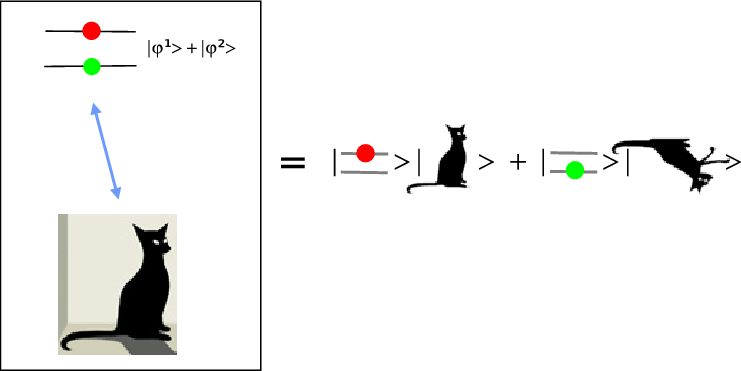
\includegraphics[width=10cm,height=5cm]{cats.png}
    \caption{Schrödinger's Cat's Probabilities Representation[2]}
    \label{fig:w_logic}
\end{figure}
\paragraph{}Before the box is opened and the system is observed, the atom exists in a superposition of both decayed and undecayed states. According to the principles of quantum mechanics, this superposition extends to the entire system, meaning that the cat is simultaneously alive and dead until observed. Only when the box is opened and the system is measured does the cat’s state collapse into one of the two possibilities—alive or dead.

This thought experiment highlights the peculiar nature of quantum superposition, where particles can exist in multiple states at once, a phenomenon not observed in the classical world. The Schrödinger cat is therefore a metaphor to illustrate the counterintuitive aspects of quantum mechanics, particularly the role of measurement in determining the state of a quantum system.
\subsection{The Role of Superposition in Quantum Computing}
In a classical system, a state can exist only or not exist. It is about living or dying, sleeping or being awake, going to work or not, etc. In other words, in the world, which is a classical system, something can either exist or not exist. This situation is the same as in the classical computers. However, in quantum computers, superposition makes both situations possible at the same time. The best example that explains the contribution of this situation is the labyrinth example.
In classical computers, finding the exit of a maze involves progressing step by step through a set of possibilities. The computer tries one path at a time and if it encounters a dead end, it backtracks and tries the next possible path. This process can take a long time if the maze is complex and branching because the classical computer must test each path sequentially. This represents the limitation of a classical computer that can operate only on one possibility at a time.

However, in \textbf{quantum computers}, things work very differently. Thanks to quantum superposition, a qubit can exist in multiple states at once. This means that a quantum computer can explore multiple paths of the maze simultaneously. In superposition, the quantum computer can attempt both correct and incorrect paths at the same time. Therefore, it can effectively search the entire maze in parallel, dramatically reducing the time required to find the exit.

\subsubsection*{Difference Between Classical and Quantum Computers}

\begin{itemize}
    \item \textbf{Classical Computer}: The classical computer tries each path in the maze one by one. At each step, it selects a path, and if it reaches a dead end, it backtracks and tries the next possibility. This process is sequential.
    
    \item \textbf{Quantum Computer}: Due to the superposition property, a quantum computer can test all paths simultaneously. This allows it to explore the maze in parallel and find the exit much faster.
\end{itemize}

This example demonstrates how superposition allows quantum computers to perform \textbf{parallel computations}, unlike the \textbf{serial processing} of classical computers. While a classical computer must try every possibility one after the other, a quantum computer can explore multiple possibilities at once, leading to much faster problem solving capabilities.
\subsection{Applications of Quantum Computers}

Quantum computers hold the potential to revolutionize various fields through their unique computational abilities. Here are some key applications:

\begin{itemize}
    \item \textbf{Cryptography:} Quantum computers can potentially break widely used encryption schemes, such as RSA, by efficiently factoring large numbers. However, they also enable the development of quantum-resistant cryptographic methods, which are essential for securing future communications.
    
    \item \textbf{Optimization:} Many real-world problems, such as route planning, scheduling, and resource allocation, involve finding the optimal solution among many possibilities. Quantum computers can solve these problems more efficiently using algorithms like the Quantum Approximate Optimization Algorithm (QAOA).
    
    \item \textbf{Drug Discovery:} Quantum computers can simulate molecular structures and interactions with high precision, which is valuable for discovering new drugs and materials. This capability could accelerate the development of treatments for complex diseases.
    
    \item \textbf{Machine Learning:} Quantum machine learning algorithms can process and analyze large datasets more efficiently than classical algorithms. Techniques such as quantum support vector machines and quantum neural networks offer the potential to enhance pattern recognition and data analysis.
    
    \item \textbf{Material Science:} Quantum computers can model complex materials and chemical reactions, enabling the discovery of new materials with specific properties. This has implications for developing advanced materials for electronics, energy storage, and more.

    \item \textbf{Security Simulations: } The vehicles that are manufactured (planes, cars, trains, etc.) need to be tested for safety. However, companies have calculated that doing these on computers is more expensive than doing them physically. If they could use quantum computers, they would have much shorter calculation times with more parameters and much lower costs.
\end{itemize}
These are just some of the uses that are currently being anticipated. But it is difficult to predict what the future holds. For example, when the first classic computers were produced, it was not thought that they could play thousands of games.


Quantum gates are pivotal in achieving the remarkable performance of quantum computers in various applications. They enable the manipulation and control of qubits, the fundamental units of quantum information, through unitary transformations. This capability is crucial for implementing quantum algorithms that take advantage of the unique properties of quantum mechanics, such as superposition and entanglement. Quantum gates facilitate the creation and maintenance of these quantum states, allowing quantum computers to perform complex calculations that classical computers struggle with. By orchestrating sequences of quantum gates, quantum algorithms can efficiently tackle problems in cryptography, optimization, drug discovery, machine learning, and material science. The efficiency and power of quantum computers in these domains are fundamentally rooted in the precise operation of quantum gates, which ensure that quantum mechanical principles are accurately harnessed to achieve unparalleled computational performance.
\vspace{15cm}
\section{References and Citations}

\begin{itemize}
    \item \textbf{[1]}: \url{https://physicsworld.com/a/schrodingers-cat-makes-a-better-qubit-in-critical-regime/}
    \item \textbf{[2]}: \url{https://www.researchgate.net/figure/Illustration-of-the-Schroedingers-cat-paradox-an-atom-a-bottle-containing-a-deathly_fig2_264550002}
\end{itemize}
\section{Contact}
Feel free to contact for suggestions and questions.
\begin{itemize}
    \item \textbf{LinkedIn} \url{https://www.linkedin.com/in/emir-kaan-%C3%B6zdemir-8016442b9/}
    \item \textbf{GitHub} \url{https://github.com/emirkaanozdemr} 
\end{itemize}
\end{document}
